\documentclass[letter,12pt]{article}
\usepackage{graphicx}
\graphicspath{ {../results/} }

\begin{document}
\pagestyle{headings}
\markright{Christopher S. Sidell csidell1@umbc.edu JZ28610 -- CMSC471 Proj2}

Given the following equation:

\begin{equation}
z = \frac{sin(x^2 + 3y^2)}{0.1+r^2}
+ (x^2 + 5y^2) * \frac{e^{1-r^2}}{2},
r = \sqrt{x^2+y^2}
\end{equation}

The following three algorithms were used to optimize and find the maximum of the function. Hill climbing from random positions has a completely random output answer. The probability of it reaching the highest point is not very high. Then hill climbing with random restarts between -2.5 and 2.5 for about 20 times. The third test is simulated annealing with the probability function of $ e^{\frac{new-current}{temperature}} $ between the same range as before.

The results set:

\begin{center}
 \begin{tabular}{c c c}
 \hline
 Name & Highest Point & Time  \\ [0.5ex]
 \hline\hline
 Hill Climbing & unreliable & 0.0588  \\
 \hline
 Hill Climb with Restart & 3.7280095530220976 & 0.7496 \\
 \hline
 Simulated Annealing & 3.596124616456771 & 0.0027 \\
 \hline
\end{tabular}
\end{center}

The Hill Climbing without random restarts is just an example of getting lucky. A good path straight to one of the highest points is very rare in this case. Hill climbing with random restarts sometimes gets lucky and follows the path straight up or get stuck in a valley. The graphs generated below show a good example of how each path each iteration took.

Simulated Annealing more often than not will get the highest and is even quicker than the hill climbing. Given the random restarts not always getting the highest and taking more time, hill climbing can be assumed that it will more often than not produce results that are not favorable. Whereas simulated annealing gives the highest within a shorter amount of time. So in a simple conclusion the simulated annealing algorithm is the best. Below you can see the example graphs in 3D space of the paths taken by each algorithm. Running the python code will result in an interactive version of the graph.

In the results however hill climbing with random results produced the highest result. This was just one of the cases where it got the highest, more often than not it was lower.

The graphs show three dimensions of x, y, and z (height). The colors are each iteration taken. The other graph is the algorithm plotted on top of the wireframe of what the function looks like

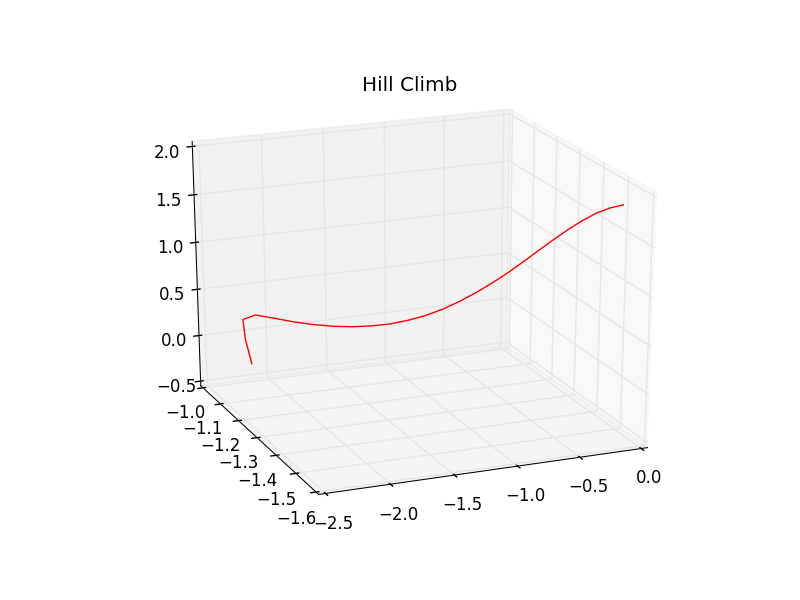
\includegraphics[scale=0.35]{hill_climb}
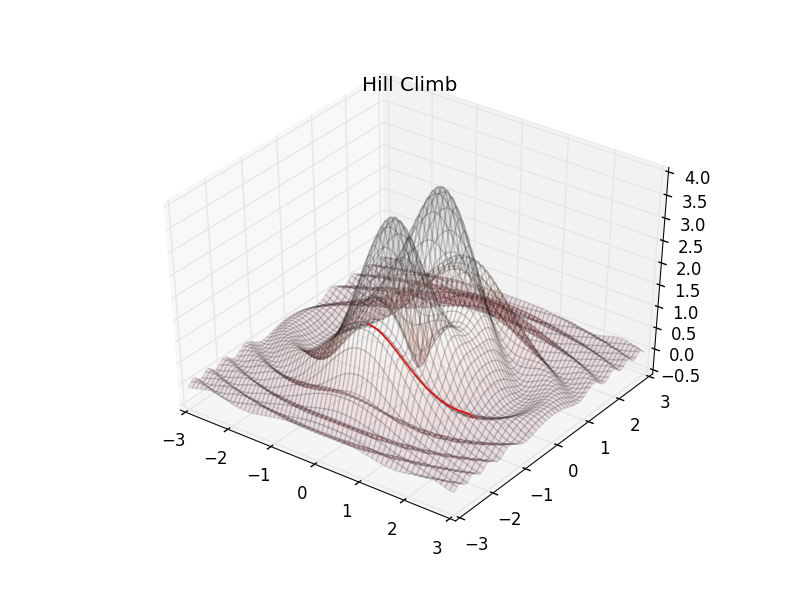
\includegraphics[scale=0.35]{hill_climb_graph}
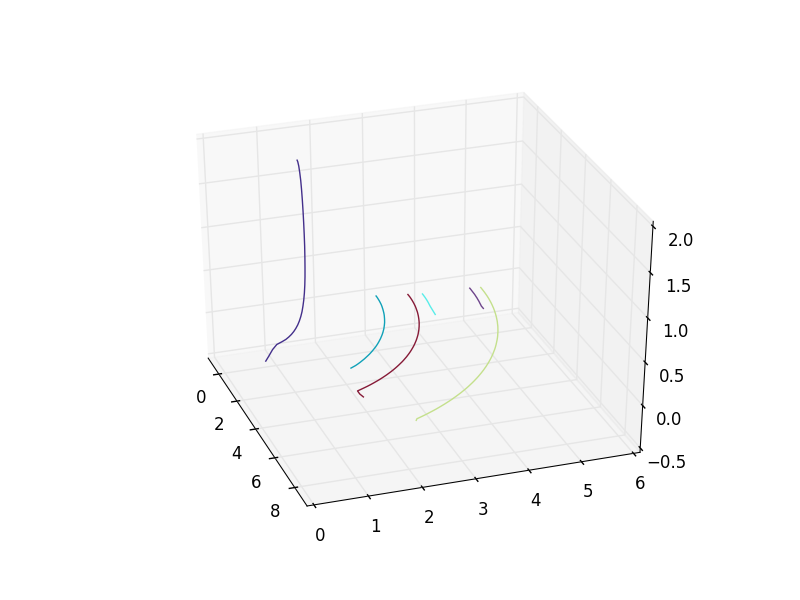
\includegraphics[scale=0.35]{hill_climb_random}
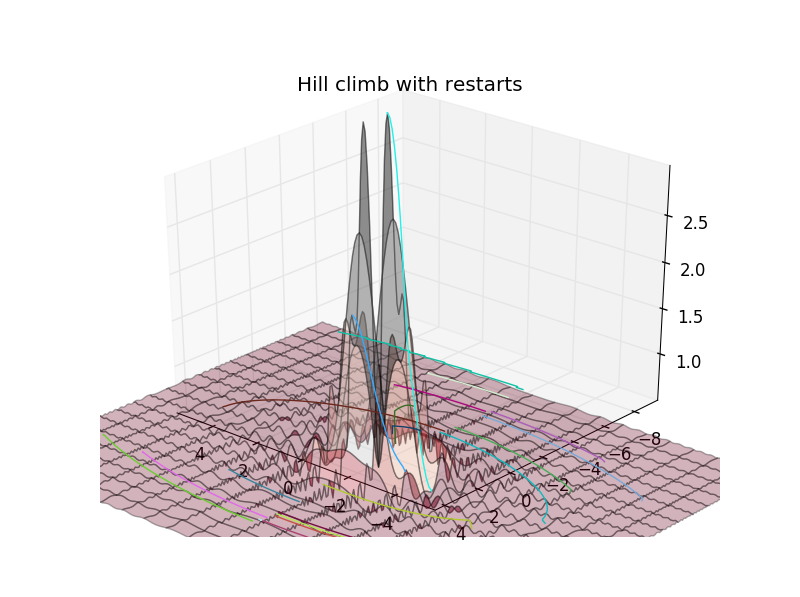
\includegraphics[scale=0.35]{hill_climb_random_graph}
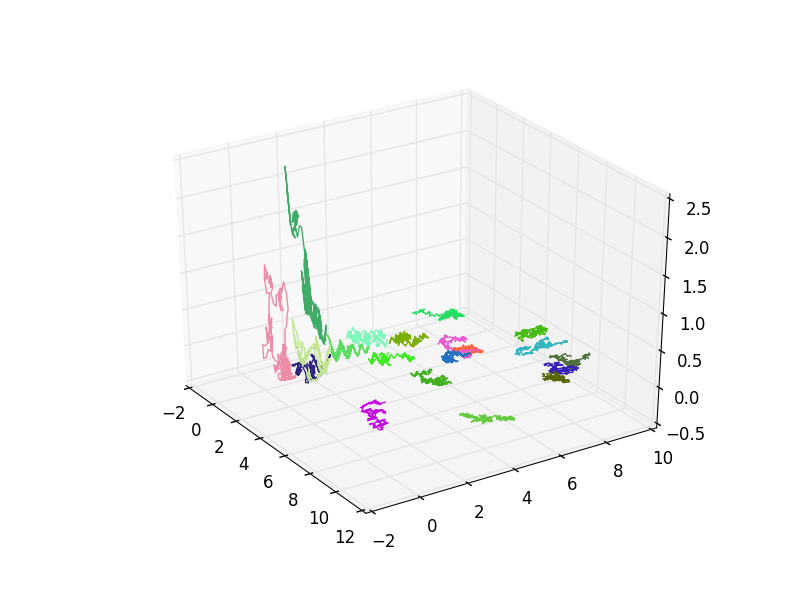
\includegraphics[scale=0.35]{simulated_annealing}
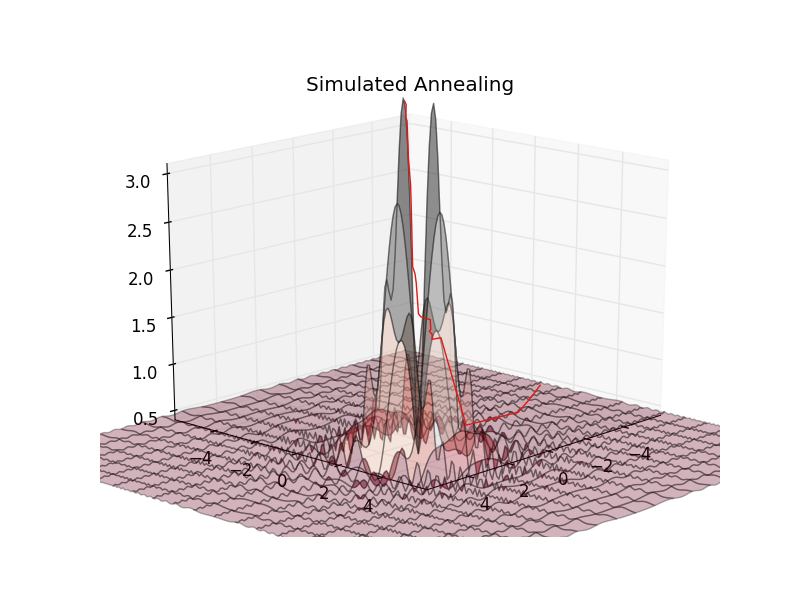
\includegraphics[scale=0.35]{simulated_annealing_graph}

\end{document}